\begin{frame}
  \frametitle{Alice is surfing...}
  \begin{block}{}
    \vskip -1.2cm
    \begin{figure}[t]
      \centering
      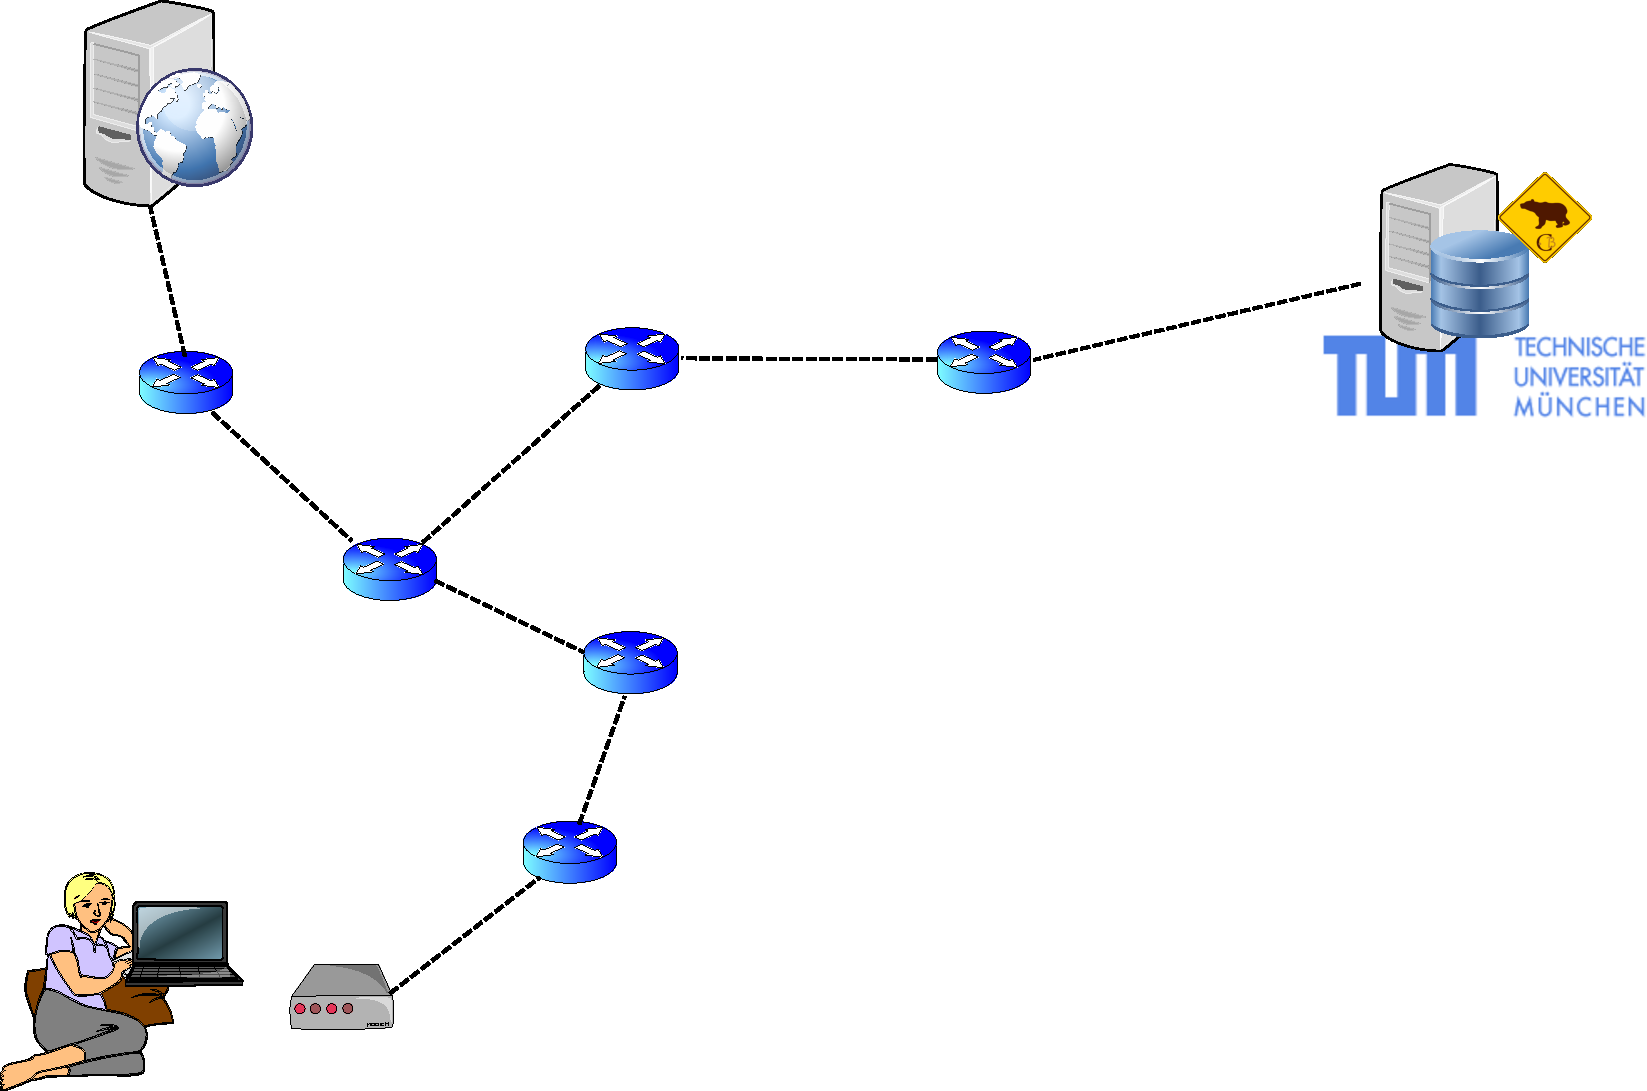
\includegraphics[scale=.36]{figures/reporting}
    \end{figure}
  \end{block}
\end{frame}

\begin{frame}
  \frametitle{Man-in-the-middle}
  \begin{block}{}
    \vskip -1.1cm
    \begin{figure}[t]
      \centering
      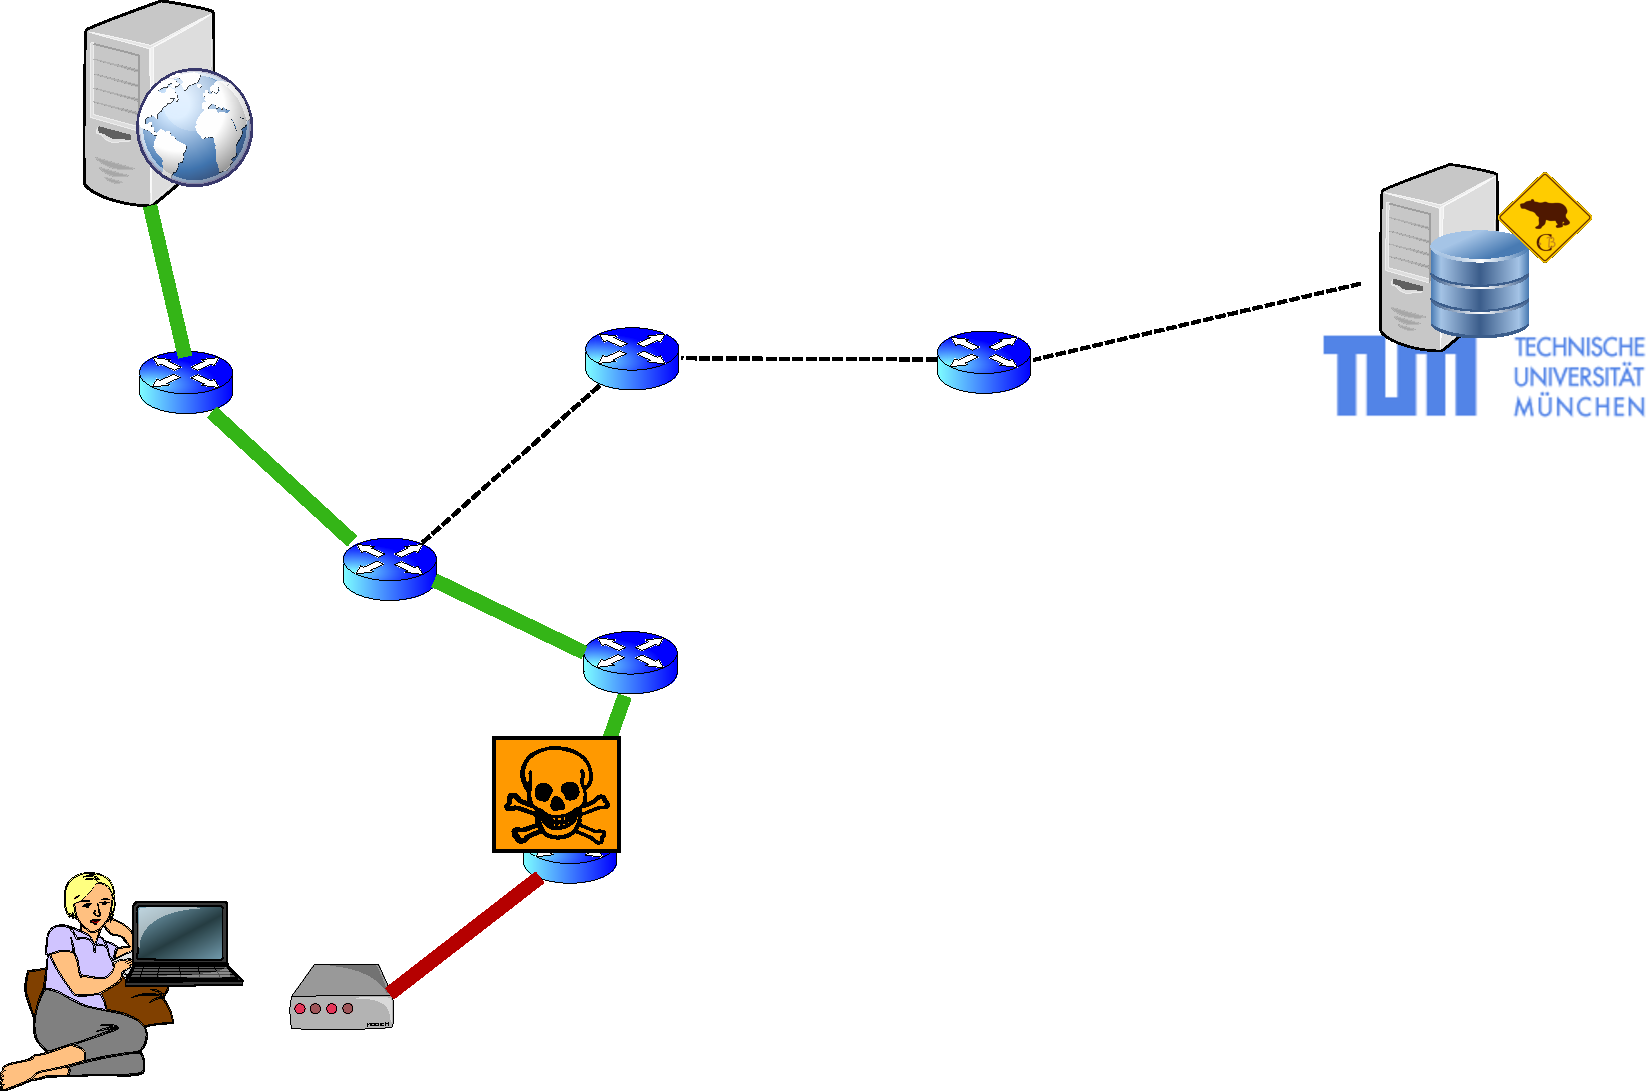
\includegraphics[scale=.36]{figures/reporting-2-attacked}
    \end{figure}
  \end{block}
\end{frame}

\begin{frame}
  \frametitle{Alice queries Crossbear}
  \begin{block}{}
    \vskip -1.2cm
    \begin{figure}[t]
      \centering
      \includegraphics[scale=.36]{figures/reporting-3-querying}
    \end{figure}
  \end{block}
  \vskip -.5cm
  \begin{block}{\small NB: SSL-secured connection, server cert hard-coded}\end{block}
\end{frame}

\begin{frame}
  \frametitle{Crossbear checks the server}
  \begin{block}{}
    \vskip -1.1cm
    \begin{figure}[t]
      \centering
      \includegraphics[scale=.36]{figures/reporting-4-checking}
    \end{figure}
  \end{block}
\end{frame}


\begin{frame}
  \frametitle{Crossbear reports result}
  \begin{block}{}
    \vskip -1.2cm
    \begin{figure}[t]
      \centering
      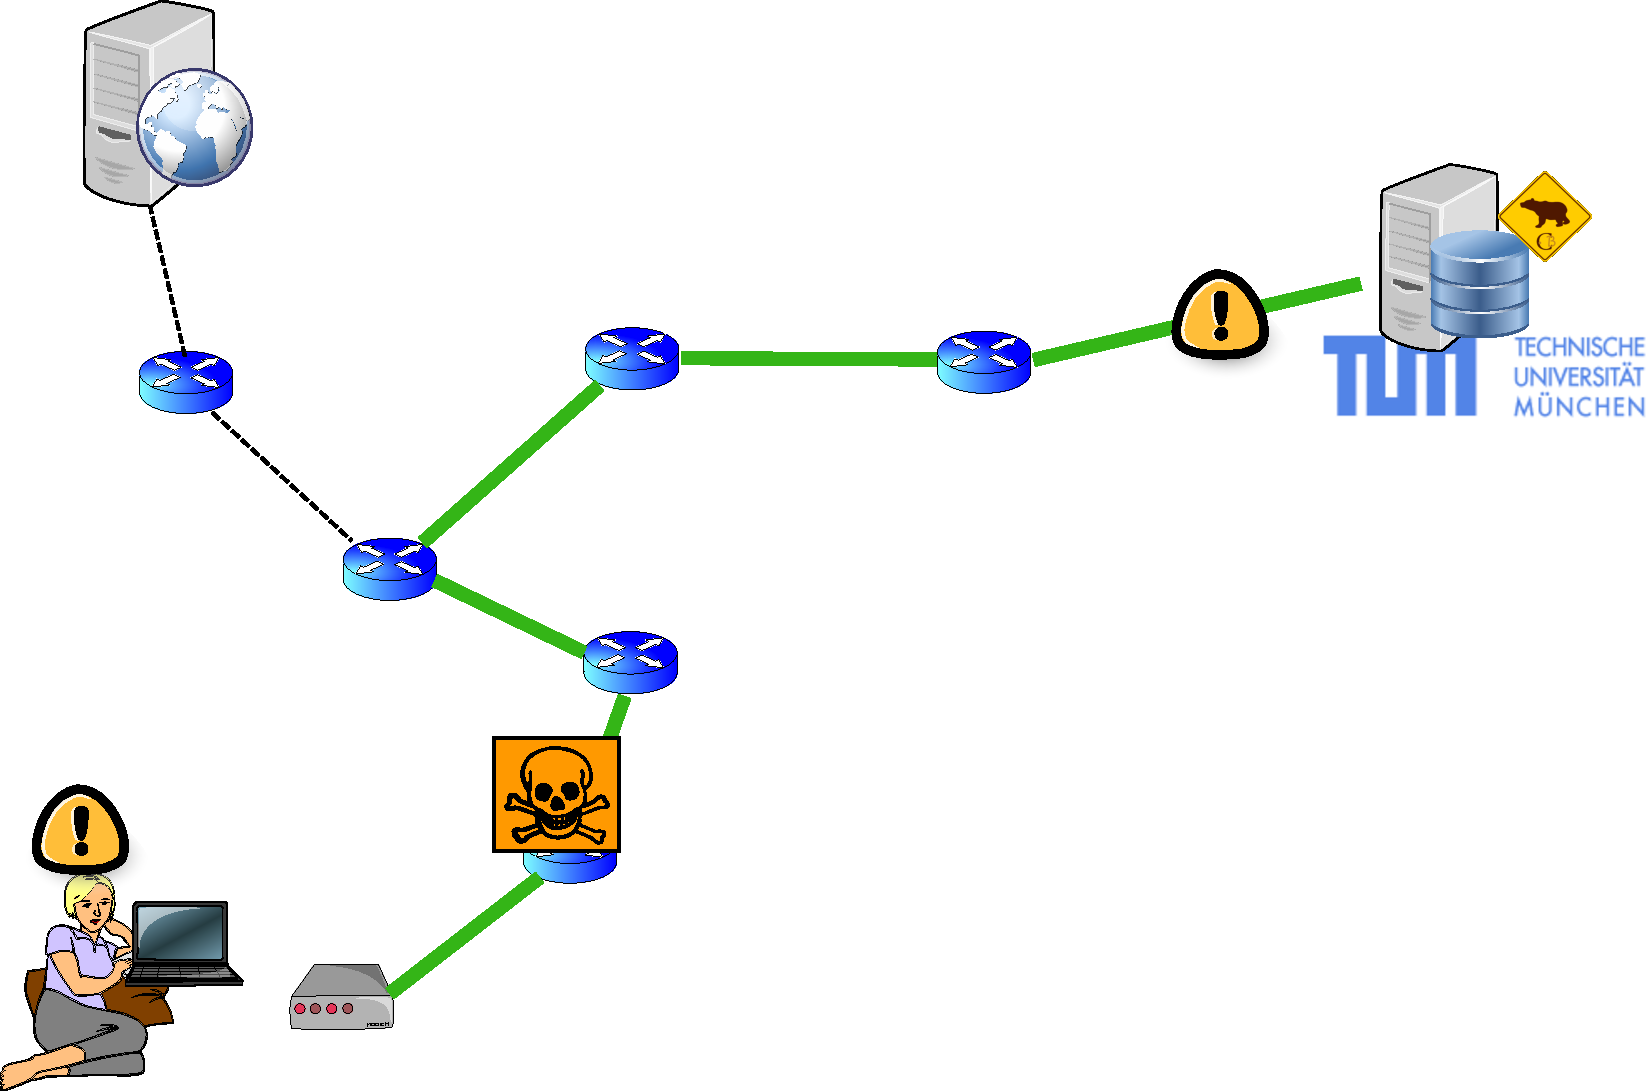
\includegraphics[scale=.36]{figures/reporting-5-feedback}
    \end{figure}
  \end{block}
\end{frame}


\begin{frame}
  \frametitle{Alice traceroutes to server}
  \begin{block}{}
    \vskip -1.1cm
    \begin{figure}[t]
      \centering
      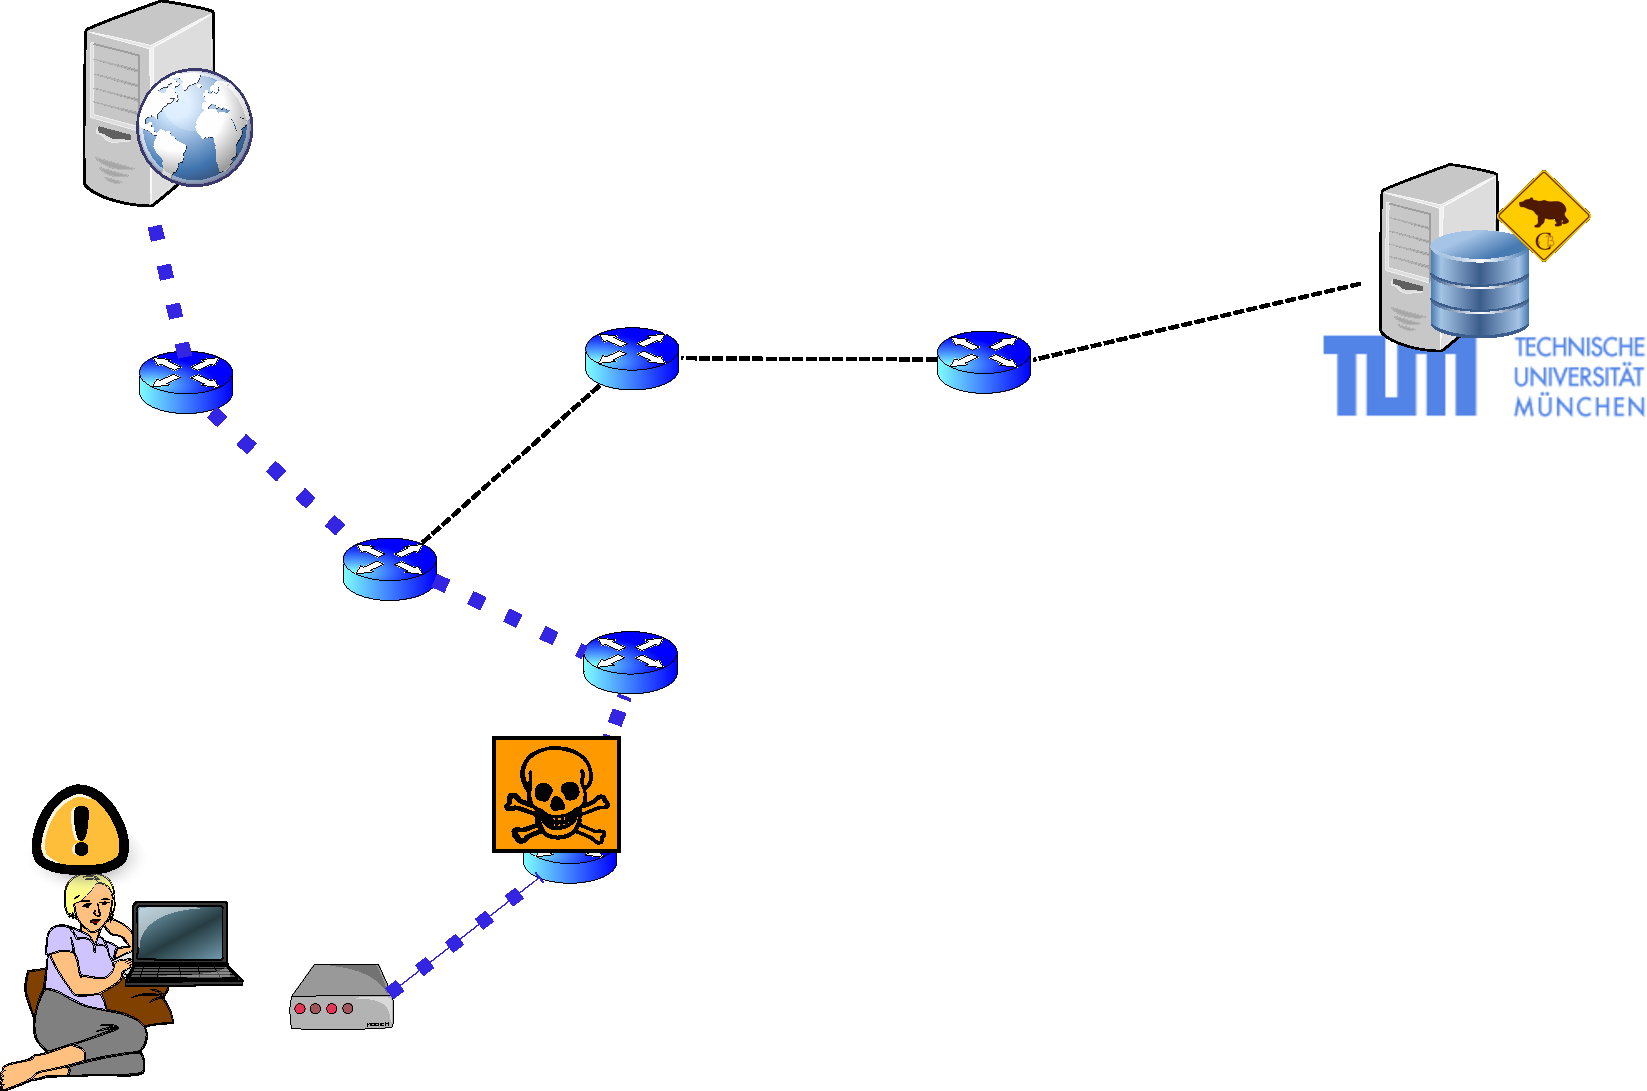
\includegraphics[scale=.36]{figures/reporting-6-hunting}
    \end{figure}
  \end{block}
\end{frame}


\begin{frame}
  \frametitle{Alice reports to Crossbear}
  \begin{block}{}
    \vskip -1.2cm
    \begin{figure}[t]
      \centering
      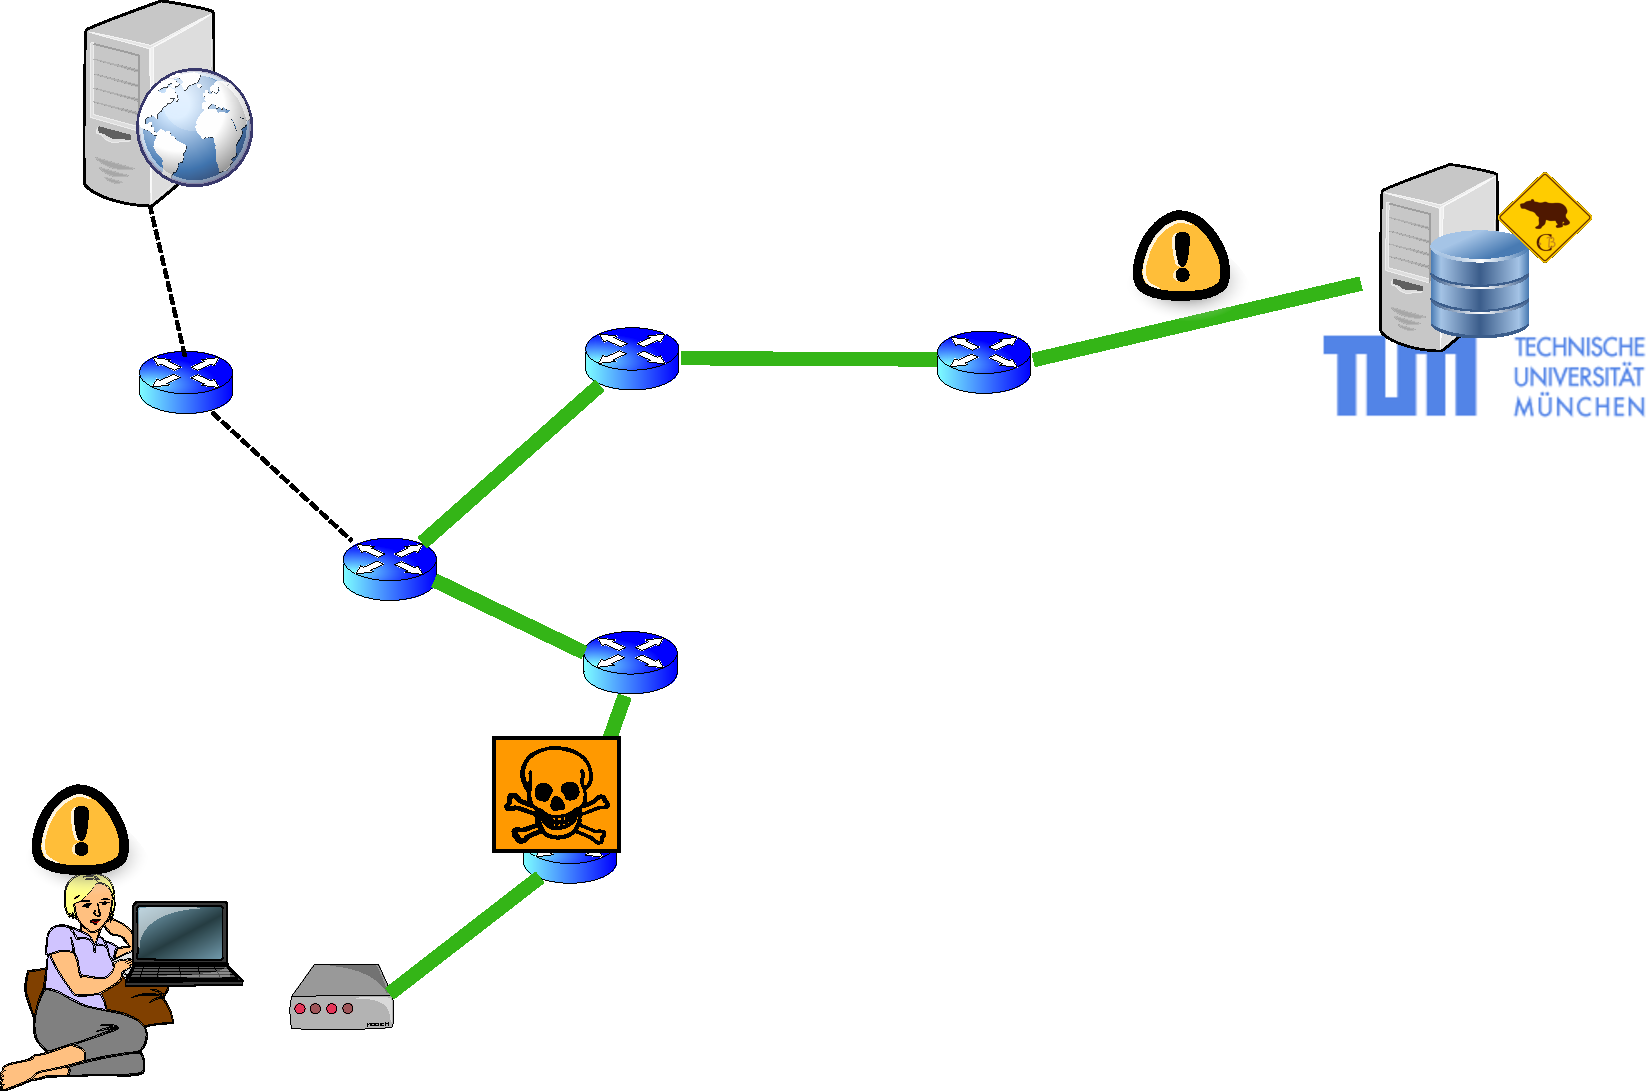
\includegraphics[scale=.36]{figures/reporting-7-huntingreport}
    \end{figure}
  \end{block}
\end{frame}

\begin{frame}
  \frametitle{Distribute hunting tasks}
  \begin{block}{}
    \vskip -1.2cm
    \begin{figure}[t]
      \centering
      \includegraphics[scale=.36]{figures/hunting-1-polling}
    \end{figure}
  \end{block}
\end{frame}

\begin{frame}
  \frametitle{Bob goes hunting}
  \begin{block}{}
    \vskip -1.2cm
    \begin{figure}[t]
      \centering
      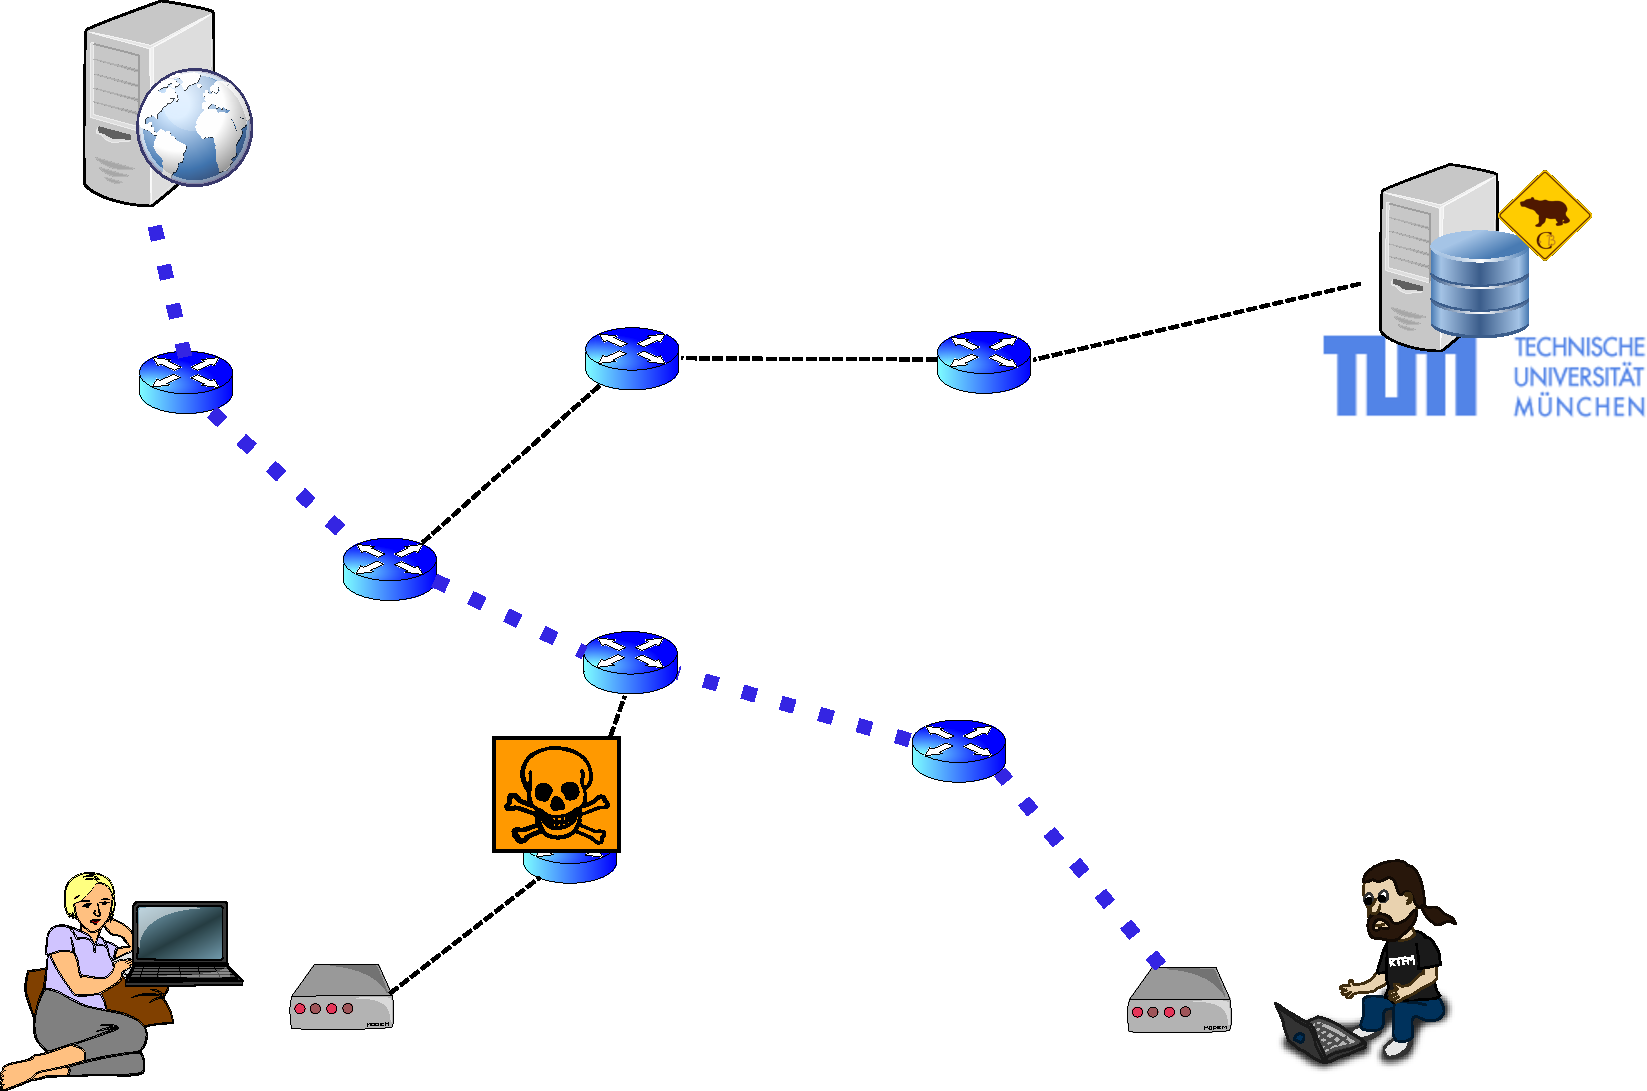
\includegraphics[scale=.36]{figures/hunting-2-hunting}
    \end{figure}
  \end{block}
\end{frame}

\begin{frame}
  \frametitle{Bob reports}
  \begin{block}{}
    \vskip -1.2cm
    \begin{figure}[t]
      \centering
      \includegraphics[scale=.36]{figures/hunting-3-reporting}
    \end{figure}
  \end{block}
\end{frame}

\begin{frame}
  \frametitle{There are many Bobs}
  \begin{block}{}
    \vskip -1.2cm
    \begin{figure}[t]
      \centering
      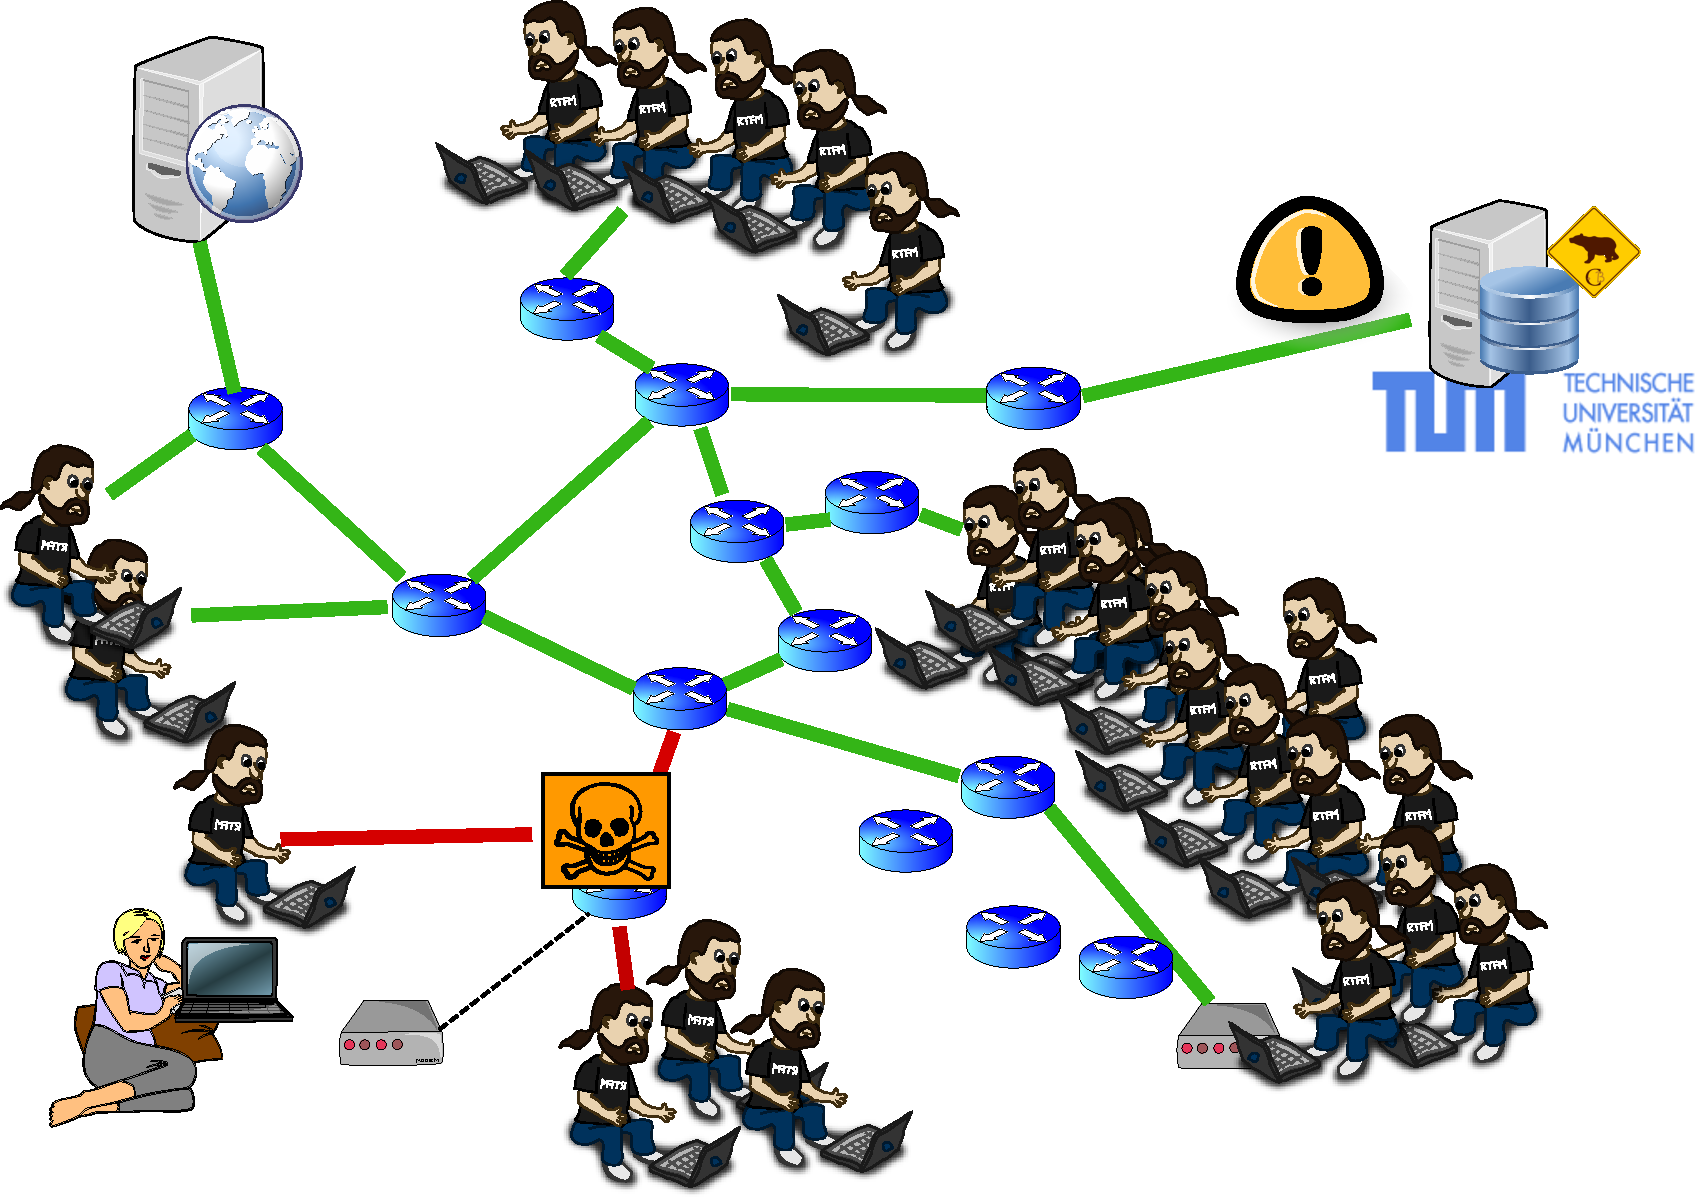
\includegraphics[scale=.36]{figures/hunting-4-manyreporting}
    \end{figure}
  \end{block}
\end{frame}

\begin{frame}
  \frametitle{Components}
  \begin{block}{Server: store and analyse}
    \begin{itemize}
    \item Crossbear server at TU M{\"u}nchen, Germany
    \item Additionally uses Convergence project's notaries
    \item Server cert hard-coded into client!
    \end{itemize}
  \end{block}
  \begin{block}{Clients}
    \begin{itemize}
    \item Firefox plugin (detection and localisation)
    \item Standalone hunting implementation (localisation only)
    \item OONIBear client (localisation only)
    \end{itemize}
  \end{block}
\end{frame}

\begin{frame}
  \frametitle{Additional data raised}
  \begin{block}{We also determine on server-side:}
    \begin{itemize}
    \item CAs used in certificate chain ($\rightarrow$ CA continuity)
    \item AS number of hosts in traceroute \\ ($\rightarrow$ Frequent
      reports about certain ASes?)
    \item Geo data: location of hosts in traceroute \\ ($\rightarrow$ Traversed countries)
    \item WHOIS info
    \end{itemize}
  \end{block}

  Also: Firefox add-on for \textit{detection} and \textit{hunting}.
\end{frame}

\begin{frame}
  \frametitle{OONIbear development}
  \begin{block}{What we did:}
    \begin{itemize}
    \item Port Crossbear client to Python
    \item Implement experimental IPv6 functionality
    \item Implemented analysers to gather additional data
    \end{itemize}
  \end{block}
  \begin{block}{What we still have to do:}
    \begin{itemize}
    \item Deeper integration into OONI
    \item Build a test setup for attacks
    \item Visualization tool for hunting results
    \end{itemize}
  \end{block}
\end{frame}

\begin{frame}
  \frametitle{Visualization mockup}
  \vspace{0.1\textheight}
  \begin{figure}[t]
    \centering
    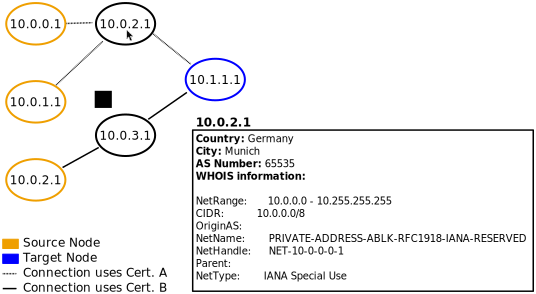
\includegraphics[width=.8\textwidth]{figures/Mockup-1}
  \end{figure}
\end{frame}

% \begin{frame}
%   \frametitle{Non-selective, close to victim client}
%   \begin{block}{}
%     \begin{figure}[t]
%       \centering
%       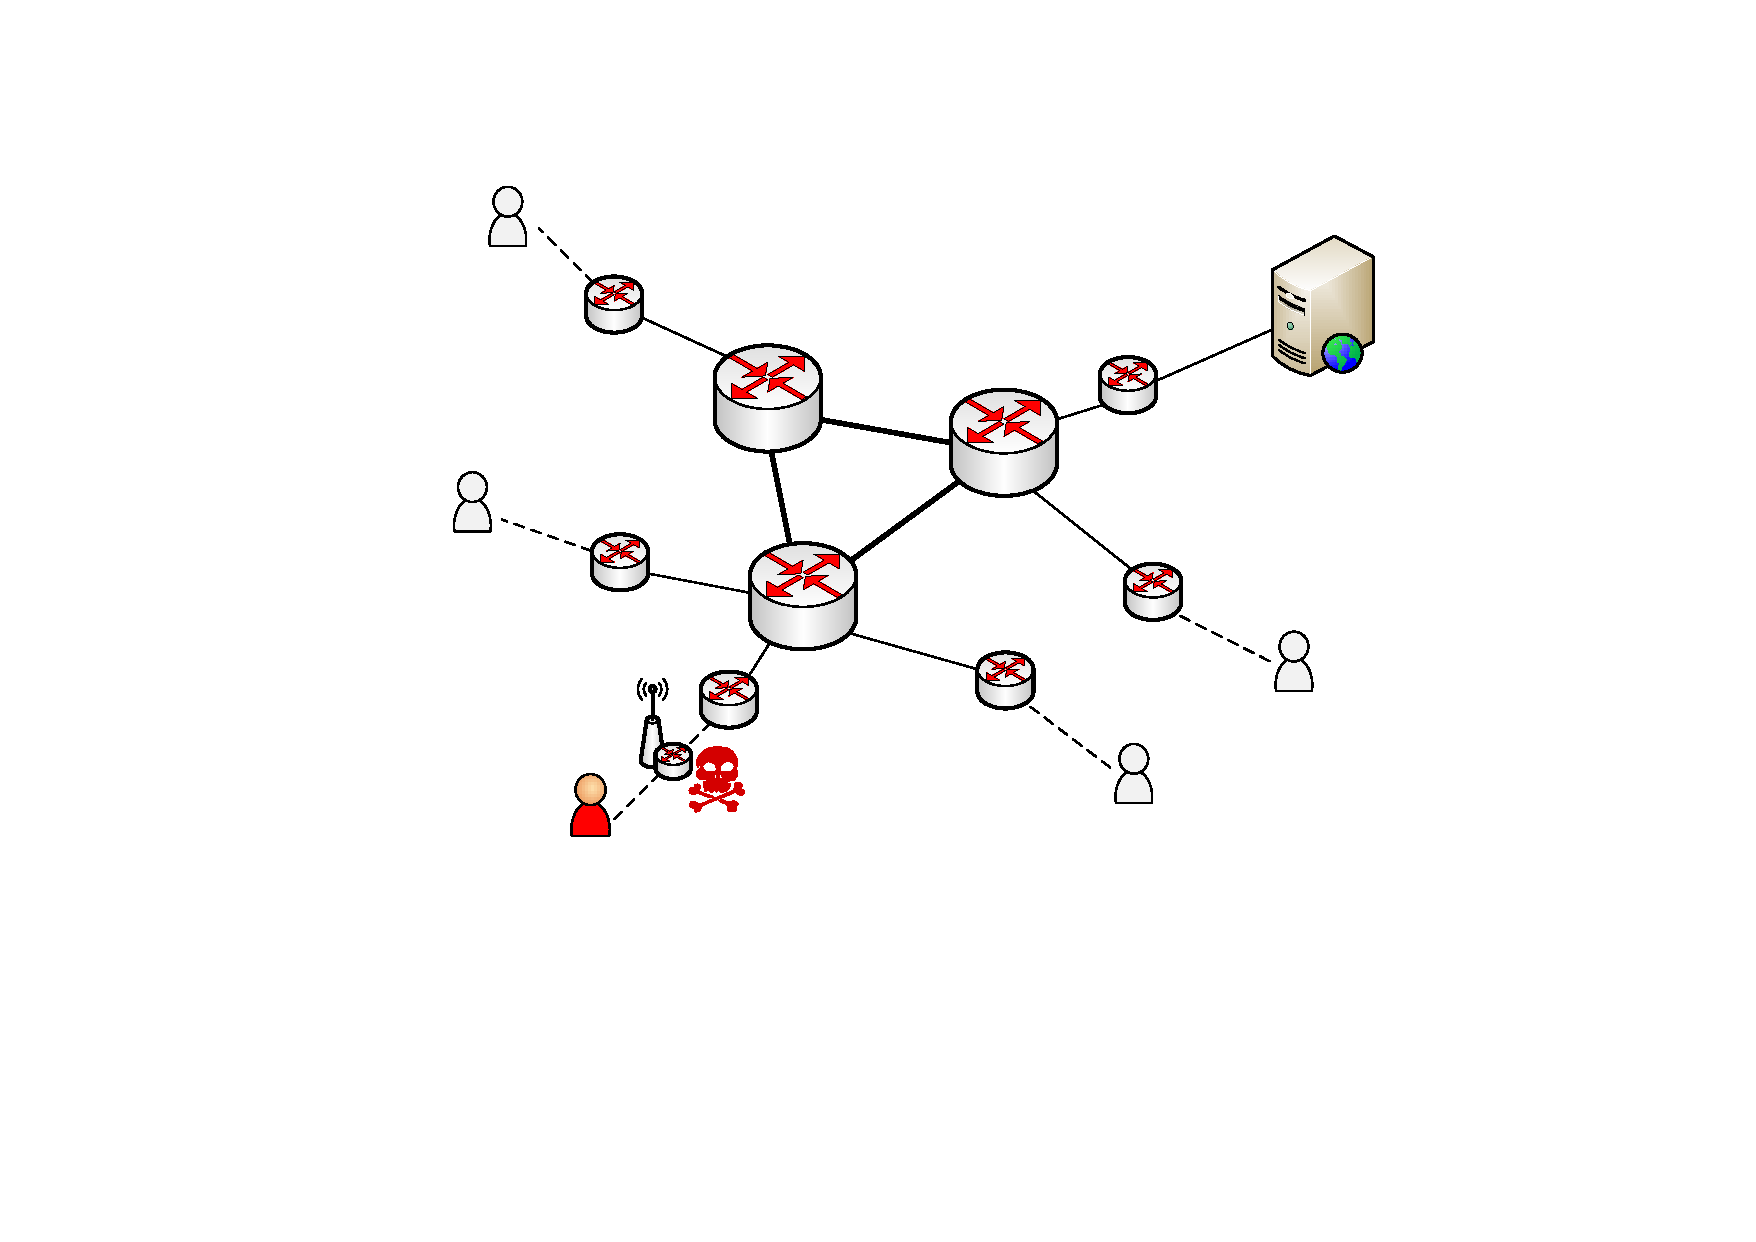
\includegraphics[scale=.5]{figures/scenario1-close-to-ap.pdf}
%     \end{figure}
%   \end{block}
% \end{frame}



% \begin{frame}
%   \frametitle{Non-selective, state-level attacker}
%   \begin{block}{}
%     \begin{figure}[t]
%       \centering
%       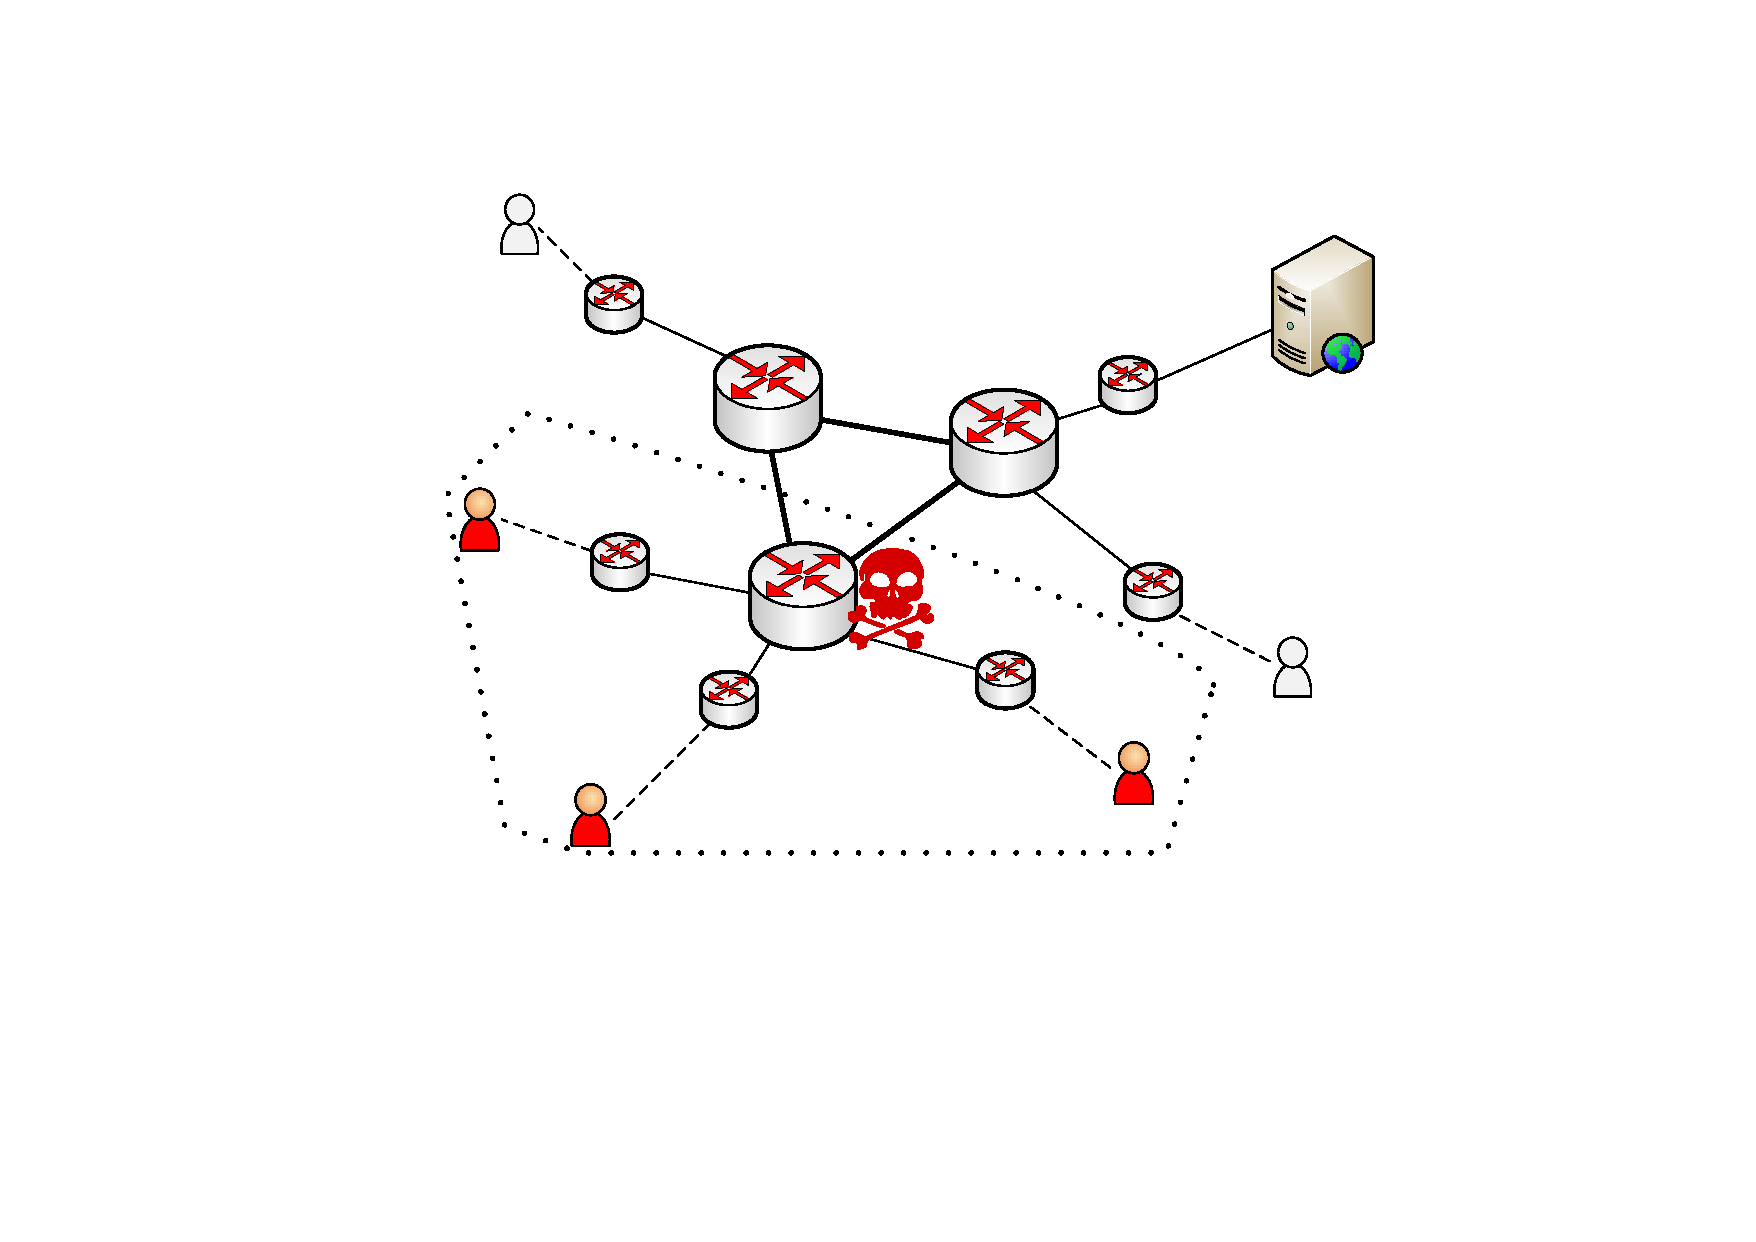
\includegraphics[scale=.5]{figures/scenario5-stateattacker-non-selective.pdf}
%     \end{figure}
%   \end{block}
% \end{frame}




% \begin{frame}
%   \frametitle{Analysis: non-selective attacker}
%   \begin{block}{Detection}
%     \begin{itemize}
%     \item Attack is detected if $\geq 1$ reports
% %     \item Attacker can only drop connections to Crossbear server
%     \end{itemize}
%   \end{block}
%   \begin{block}{Lends itself well to localisation}
%     \begin{itemize}
%     \item Get $\geq 1$ traceroute from victim,  $\geq 1$ from unpoisoned hunter 
%     \item The more, the better. The closer to intersection point, the better.
% %     \item Success depends on the number of hunters
%     \item An estimate can be given: \\ $<100$ hunters for $95\%$ accuracy on AS-level
%     \item Adaptive attackers are a problem (can't discuss here)
%     \item Full details in Crossbear research paper
%     \end{itemize}
%   \end{block}
% \end{frame}



% \begin{frame}
%   \frametitle{Number of hunters vs. success}
%   \vskip -.7cm
%   \begin{block}{}
%     \begin{figure}[t]
%       \centering
%       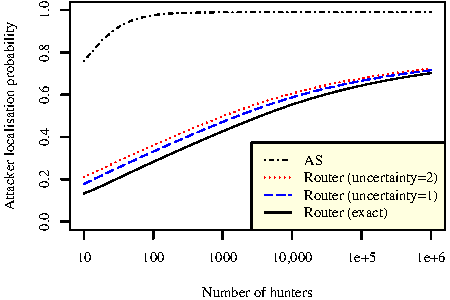
\includegraphics[scale=1.2]{figures/plot.pdf}
%     \end{figure}
%   \end{block}
%   \begin{block}{Imperfect, but given lack of data probably the best we can get.}\end{block}
% \end{frame}

\begin{frame}
  \frametitle{Thank you!}
  \vskip 1cm
  \begin{center}
    
\includegraphics[scale=0.2]{figures/question_mark.pdf}
  \end{center}
  \begin{block}{Contact}
    \begin{itemize}
    \item Twitter: @crossbearteam
    \item WWW: \texttt{https://pki.net.in.tum.de}
    \item \url{https://github.com/crossbear/Crossbear}
    \end{itemize}
  \end{block}
\end{frame}



\begin{frame}
  \frametitle{Selective attackers are a headache}
  \begin{figure}[t]
    \centering
    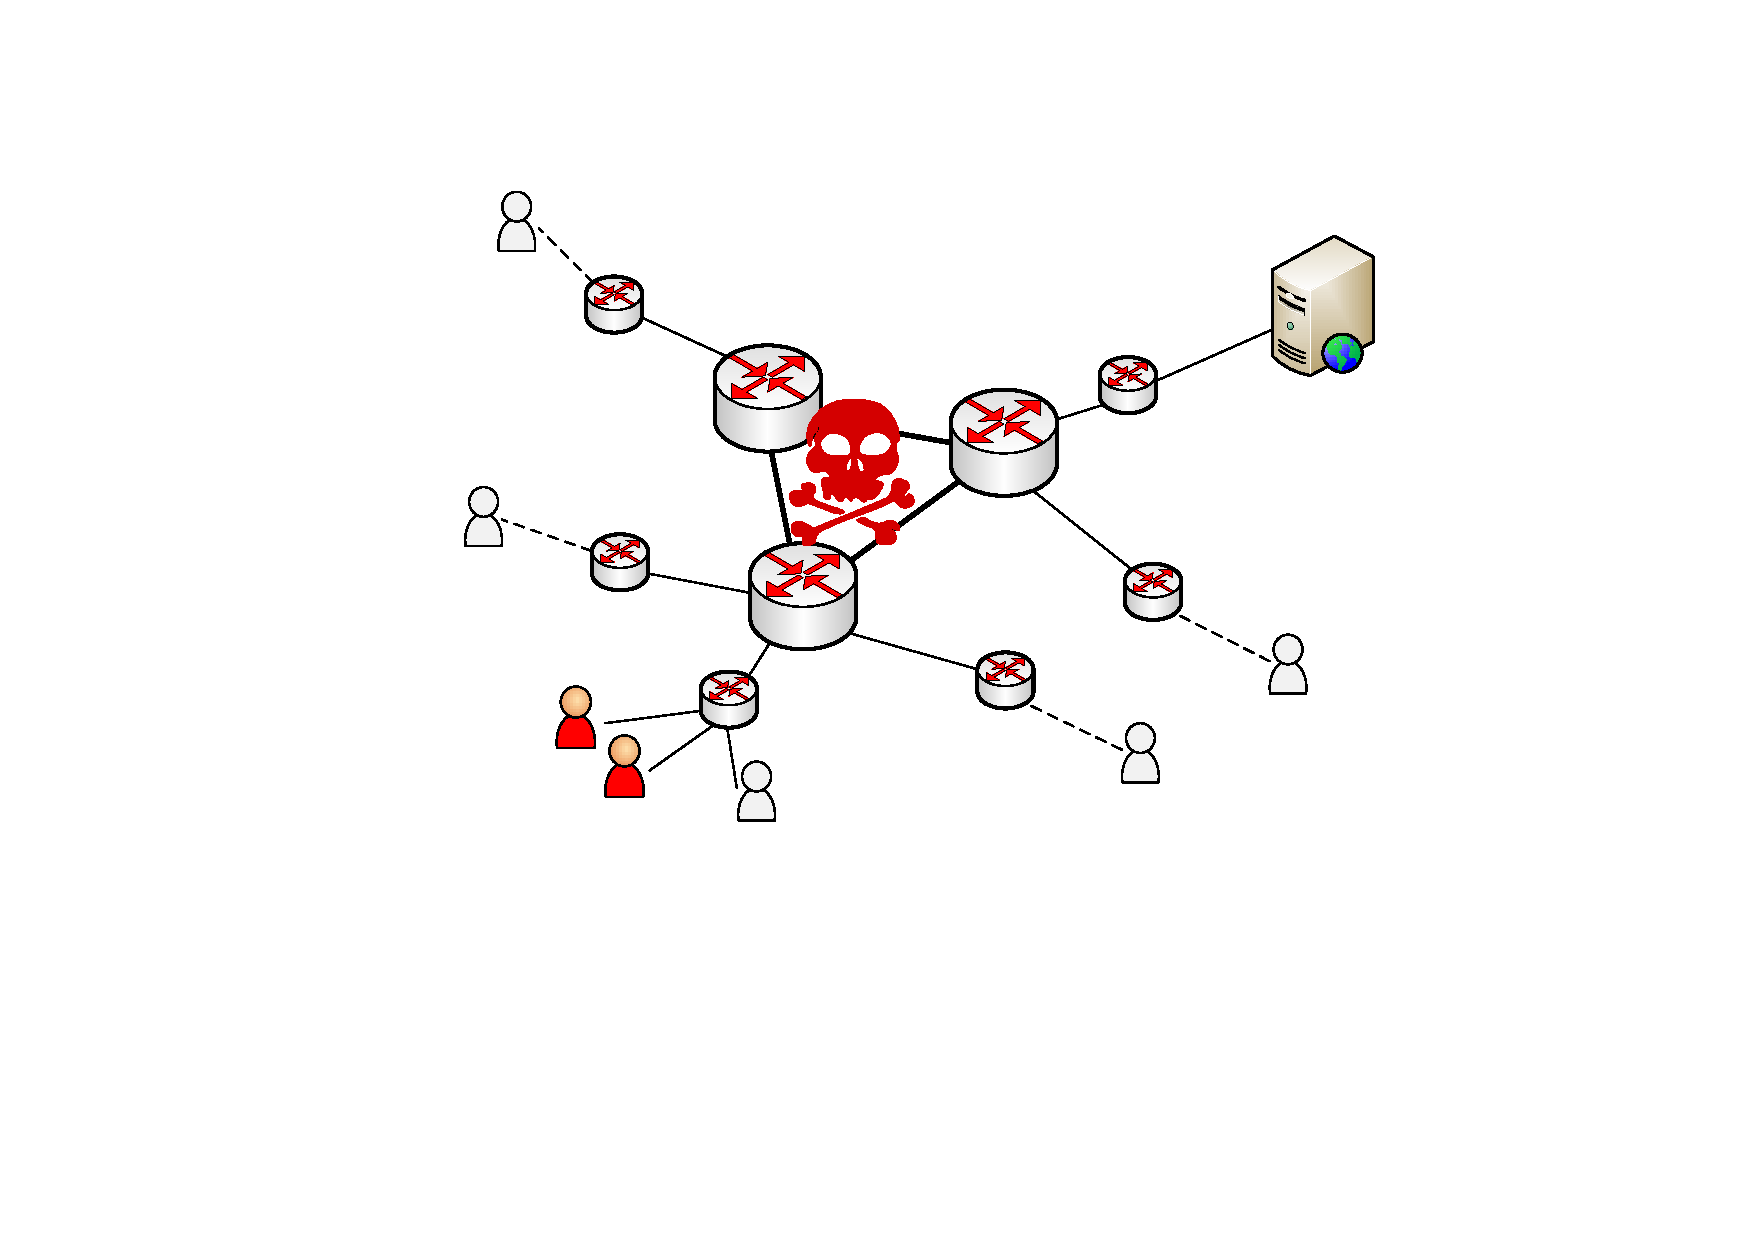
\includegraphics[scale=.3]{figures/scenario4-core-selective.pdf}
  \end{figure}
  \begin{block}{Can be indistinguishable from non-selective attacks}
    \begin{itemize}
    \item \textit{Every} attack report to be checked for plausibility
    \item But attacker should leave some hints -- cannot arbitrarily spoof IP addresses
    \end{itemize}
  \end{block}
\end{frame}



\begin{frame}
  \frametitle{Other issues}
  \begin{block}{Crossbear is an open system}
    \begin{itemize}
    \item Malicious injection of data
      \begin{itemize}
      \item Clients/hunters have no ID, no authentication
      \item Attacker can eclipse real hunters in his network, too
      \item Should results in clusters of suspicious reports, though
      \end{itemize}
    \item Denial-of-service attacks
    \item It is an arms race
    \item Other detection systems are subject to same attacks
    \end{itemize}
  \end{block}
\end{frame}

%%% Local Variables:
%%% mode: latex
%%% TeX-master: "folien"
%%% End:
